\documentclass[10pt,letterpaper, onecolumn]{report}
\usepackage{amsmath}
\usepackage{amssymb}
\usepackage{listings}
\usepackage{xcolor}
\usepackage[lmargin=71pt, tmargin=0.6in]{geometry}
\usepackage{fancyhdr}
\usepackage{graphicx}
\usepackage{subcaption}
\usepackage{enumitem}

% Footer format
\pagestyle{fancy}
\fancyhead{}
\fancyfoot{}
\fancyfoot[L]{Author: Kacper Ragankiewicz, Index: 283415}
\fancyfoot[R]{\thepage}

% Syntax highlighting for Python
\definecolor{keywordcolor}{rgb}{0.58, 0.01, 0.24}
\definecolor{stringcolor}{rgb}{0.44, 0.55, 0.34}
\definecolor{commentcolor}{rgb}{0.5, 0.5, 0.5}
\definecolor{backgroundcolor}{rgb}{0.97, 0.97, 0.97}

\lstdefinestyle{myPythonStyle}{
    language=Python,
    backgroundcolor=\color{backgroundcolor},
    basicstyle=\ttfamily\small,
    keywordstyle=\color{keywordcolor}\bfseries,
    stringstyle=\color{stringcolor},
    commentstyle=\color{commentcolor}\itshape,
    numberstyle=\tiny\color{gray},
    numbersep=5pt,
    stepnumber=1,
    numbers=left,
    showstringspaces=false,
    tabsize=4,
    breaklines=true,
    frame=single,
    rulecolor=\color{black},
}

\renewcommand{\headrulewidth}{0pt}

\begin{document}

% Title
\begingroup
    \centering
    \LARGE \textbf{Complex Systems} \\
    \large CS2024/problem\_5.pdf \\[0.5em]
\endgroup

\begin{flushleft}
    \rule{\textwidth}{0.4pt} \\ % Horizontal line
    \textbf{Result}
\end{flushleft}

\begin{flushleft}
    \textbf{Task 1}
    \hfill\break
    \setlength{\parindent}{1.5em} % Adjust paragraph indentation
    \setlength{\parskip}{0.5em}   % Adjust paragraph spacing

    For "https://websites.umich.edu/~mejn/netdata/" - Zachary's karate club (karate.gml)

    \begin{figure}[htbp!]
        \centering
        \begin{subfigure}{0.45\textwidth}
            \centering
            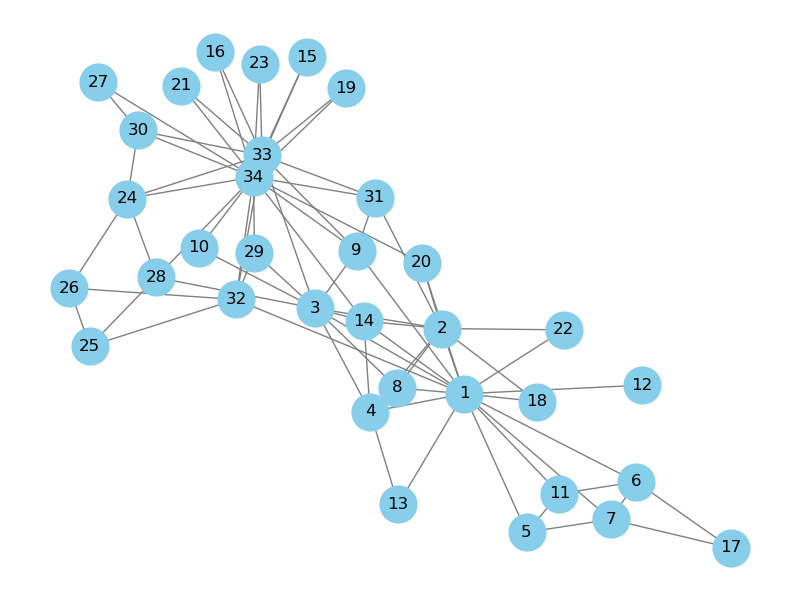
\includegraphics[width=\textwidth]{../graph.png}
            \caption{Spring layout}
        \end{subfigure}
        \hfill
        \begin{subfigure}{0.45\textwidth}
            \centering
            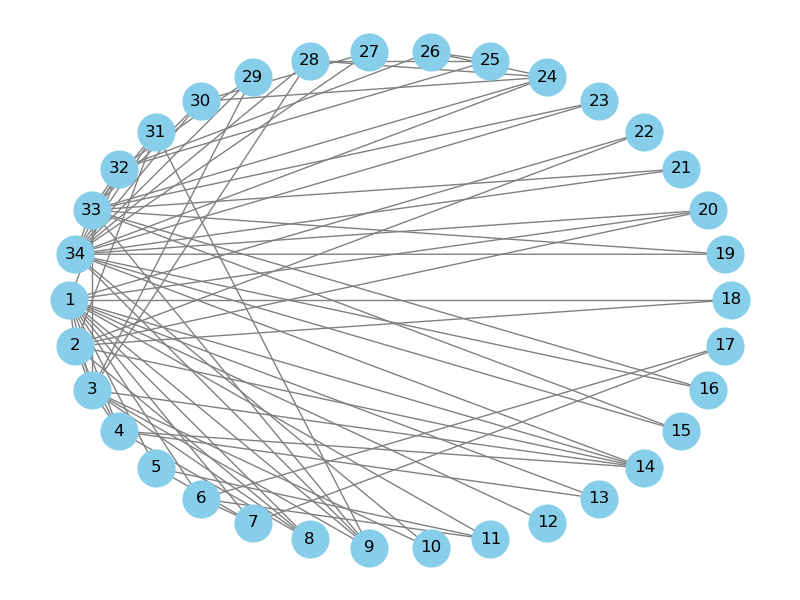
\includegraphics[width=\textwidth]{../zachary_karate_club_shell_layout.png}
            \caption{Shell layout}
        \end{subfigure}
        \caption{Nodes: 34, Edges: 78}
    \end{figure}
    
\end{flushleft}

\begin{flushleft}
    \textbf{Task 2}
    \hfill\break
    \setlength{\parindent}{1.5em} % Adjust paragraph indentation
    \setlength{\parskip}{0.5em}   % Adjust paragraph spacing

    \begin{enumerate}[label=(\alph*)]
        \item Network layout
        
        \begin{figure}[htbp!] % Positioning options: here, top, bottom, page
            \centering
            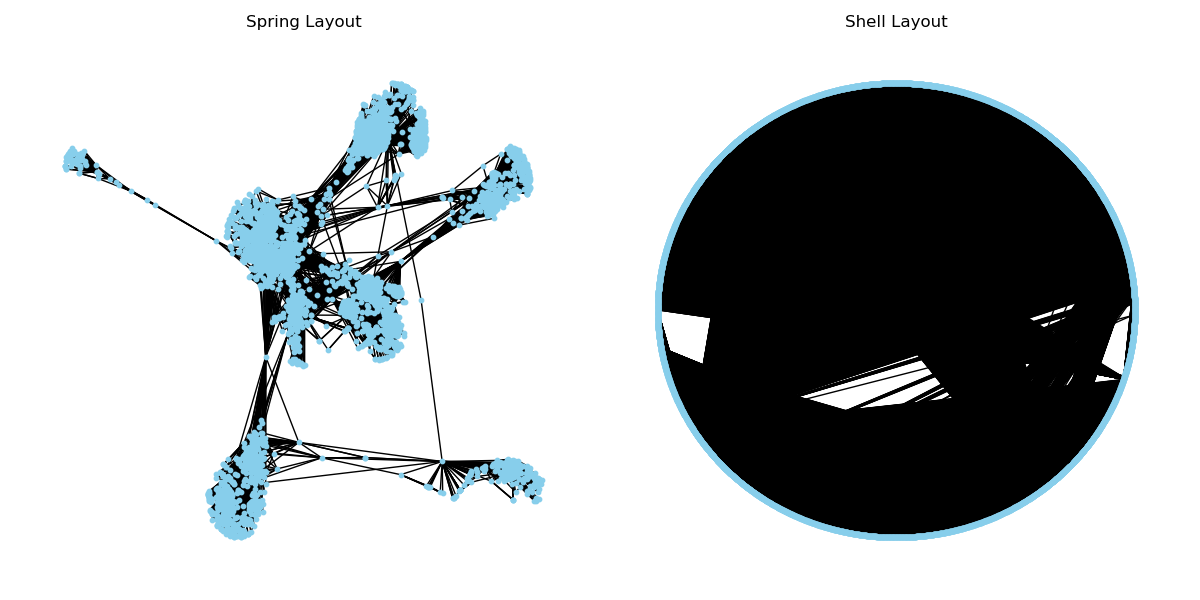
\includegraphics[width=1\textwidth]{../network_layouts.png} % Specify image file and scale
            \caption{ego-Facebook Network Layout} % Caption for the image
        \end{figure}

        \item Degree Distribution
        
        The degree of a node in a graph refers to the number of edges that are incident to it. It is evident that many nodes are connected to fewer nodes compared to others.
        \begin{figure}[htbp!] % Positioning options: here, top, bottom, page
            \centering
            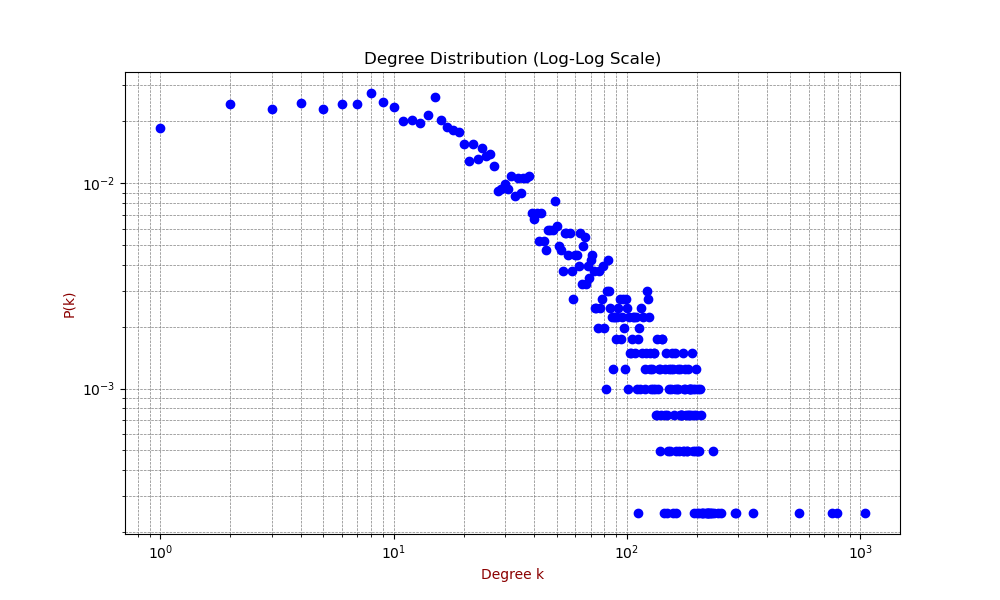
\includegraphics[width=0.49\textwidth]{../degree_distribution.png} % Specify image file and scale
            \caption{Average degree $<$ k $>$: 43.69101262688784} % Caption for the image
        \end{figure}

        \item Distribution of clustering coefficients and an average clustering coefficient.
        
        The clustering coefficient indicates the likelihood that a node's neighbors are connected to each other, forming a triangle. It quantifies the local connectivity of the node.

        \begin{figure}[htbp!] % Positioning options: here, top, bottom, page
            \centering
            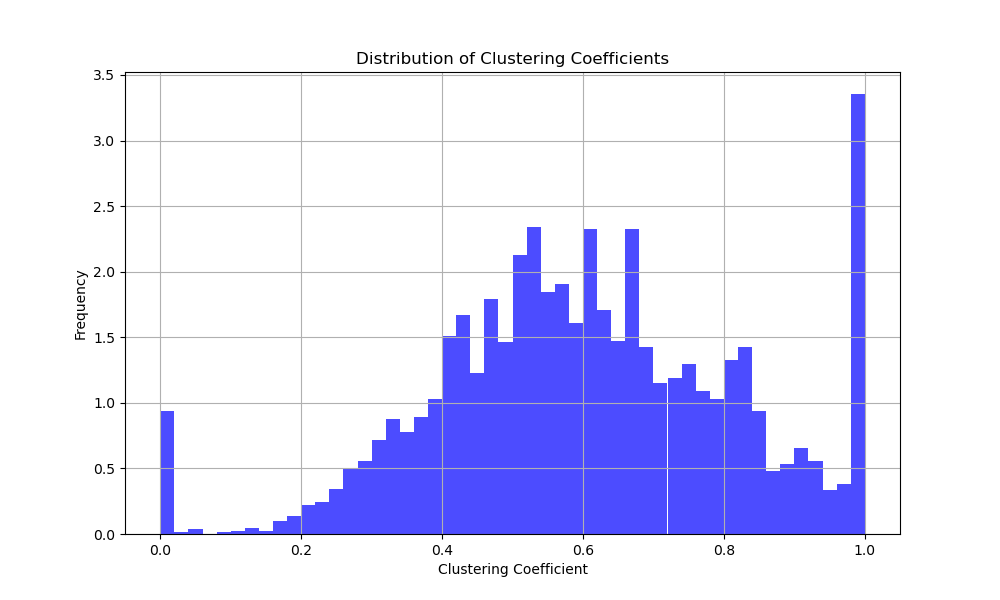
\includegraphics[width=0.49\textwidth]{../clustering_distribution.png} % Specify image file and scale
            \caption{Average Clustering Coefficient: 0.6055467186200862} % Caption for the image
        \end{figure}

        \item Distribution of the shortest paths, the diameter and the average path length

        The shortest path is the fewest edges between nodes. A histogram shows their counts, the diameter is the longest shortest path, and the average path length is their mean.
        \begin{figure}[htbp!] % Positioning options: here, top, bottom, page
            \centering
            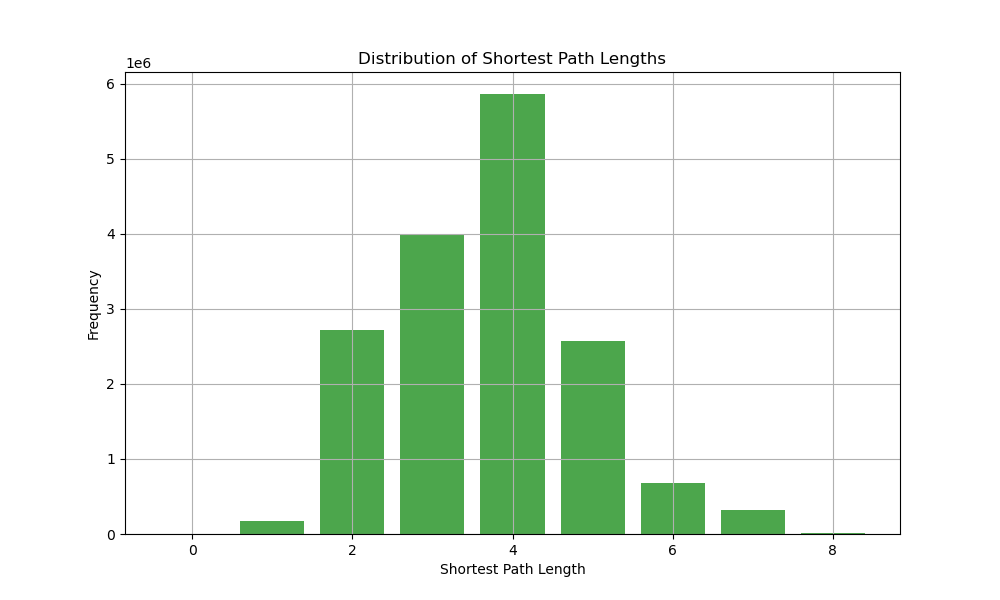
\includegraphics[width=0.49\textwidth]{../path_length_distribution.png} % Specify image file and scale
            \caption{Average Path Length: 3.691592636562027, Diameter: 8} % Caption for the image
        \end{figure}

    \end{enumerate}

\end{flushleft}

\clearpage

\begin{flushleft}
    \textbf{Task 3}
    \hfill\break
    \setlength{\parindent}{1.5em} % Adjust paragraph indentation
    \setlength{\parskip}{0.5em}   % Adjust paragraph spacing


    (a) Erdos-Renyi model G(N,L) $<$ k $>$ = 2L/N

    \begin{lstlisting}[style=myPythonStyle, caption={Erdos-Renyi model}]
def erdos_renyi(N, L):
    G = nx.Graph()
    G.add_nodes_from(range(N))

    edges = set()
    while len(edges) < L:
        u = random.randint(0, N - 1)
        v = random.randint(0, N - 1)
        if u != v and (u, v) not in edges and (v, u) not in edges:
            edges.add((u, v))

    G.add_edges_from(edges)
    return G

    \end{lstlisting}

    \begin{figure}[htbp!]
        \centering
        \begin{minipage}{0.5\textwidth} % Half the page width for the image
            \centering
            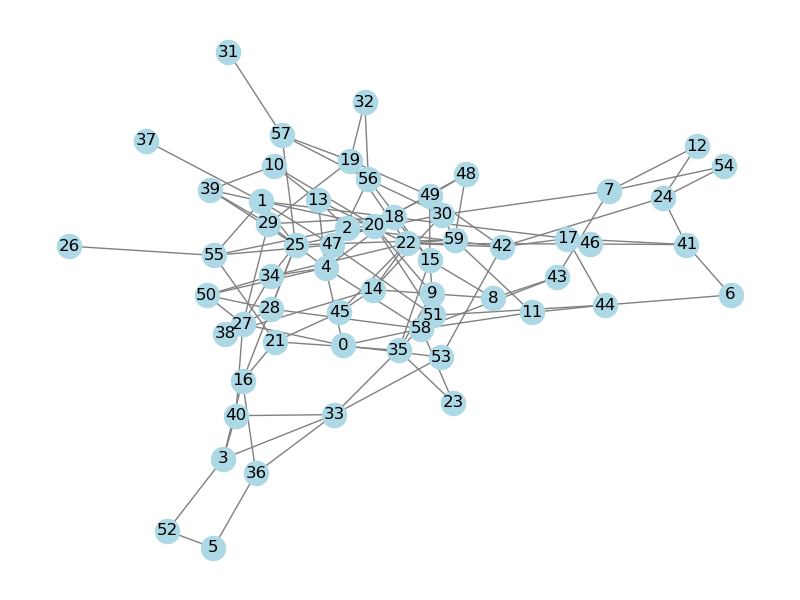
\includegraphics[width=\textwidth]{../erdos_renyi_NL.png} % Adjust the file path
            \caption{N = 60, L = 120}
            \label{fig:erdos_renyi_NL}
        \end{minipage}%
        \begin{minipage}{0.5\textwidth} % Half the page width for the statistics
            \centering
            \captionof{table}{Graph Statistics: G(N, L)}
            \begin{tabular}{|l|c|}
                \hline
                \textbf{Statistic} & \textbf{Value} \\
                \hline
                Average Degree & 6.0 \\
                Average Clustering Coefficient & 0.0525 \\
                Average Path Length & 2.706 \\
                Diameter & 5 \\
                \hline
            \end{tabular}
            \label{tab:erdos_renyi_NL_stats}
        \end{minipage}
    \end{figure}

    \begin{figure}[htbp!] % Positioning options: here, top, bottom, page
        \centering
        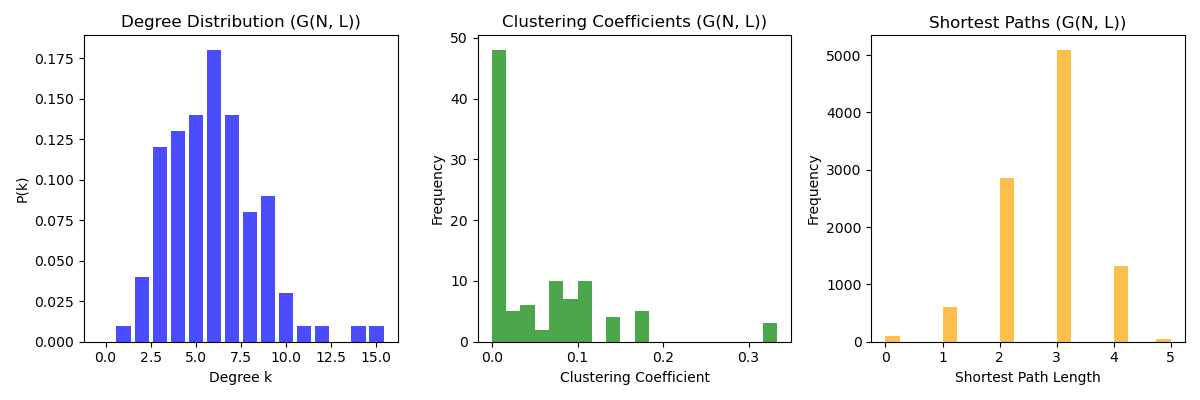
\includegraphics[width=1\textwidth]{../G(N, L)_Graph with 100 nodes and 300 edges.png} % Specify image file and scale
        \caption{N = 100, L = 300} % Caption for the image
    \end{figure}
    

    \clearpage

    (b) Erdos-Renyi-Gilbert model G(N,p) $<$ k $>$ = p(n-1)

    \begin{lstlisting}[style=myPythonStyle, caption={Erdos-Renyi model}]
# Parameters
N = 60  # Number of nodes
p = 0.25  # Probability of edge creation
G_Np = nx.erdos_renyi_graph(N, p)

# Plotting
plt.figure(figsize=(8, 6))
nx.draw(G_Np, with_labels=True, node_color='lightgreen', edge_color='gray')
plt.title(f"Erdos-Renyi-Gilbert Model G(N={N}, p={p})")
plt.savefig("erdos_renyi_gilbert_model.png")
plt.show()
     \end{lstlisting}


    \begin{figure}[htbp!]
        \centering
        \begin{minipage}{0.5\textwidth} % Half the page width for the image
            \centering
            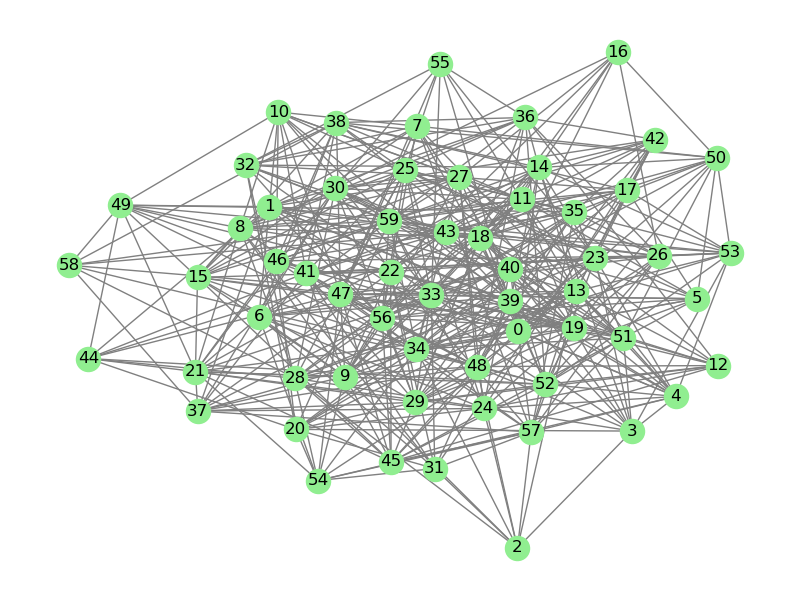
\includegraphics[width=\textwidth]{../erdos_renyi_gilbert_model.png} % Adjust the file path
            \caption{N = 60, p = 0.25}
            \label{fig:erdos_renyi}
        \end{minipage}%
        \begin{minipage}{0.5\textwidth} % Half the page width for the statistics
            \centering
            \captionof{table}{Graph Statistics: G(N, p)}
            \begin{tabular}{|l|c|}
                \hline
                \textbf{Statistic} & \textbf{Value} \\
                \hline
                Average Degree & 6.34 \\
                Average Clustering Coefficient & 0.0796 \\
                Average Path Length & 2.6372 \\
                Diameter & 5 \\
                \hline
            \end{tabular}
            \label{tab:erdos_renyi_stats}
        \end{minipage}
    \end{figure}

    \begin{figure}[htbp!] % Positioning options: here, top, bottom, page
        \centering
        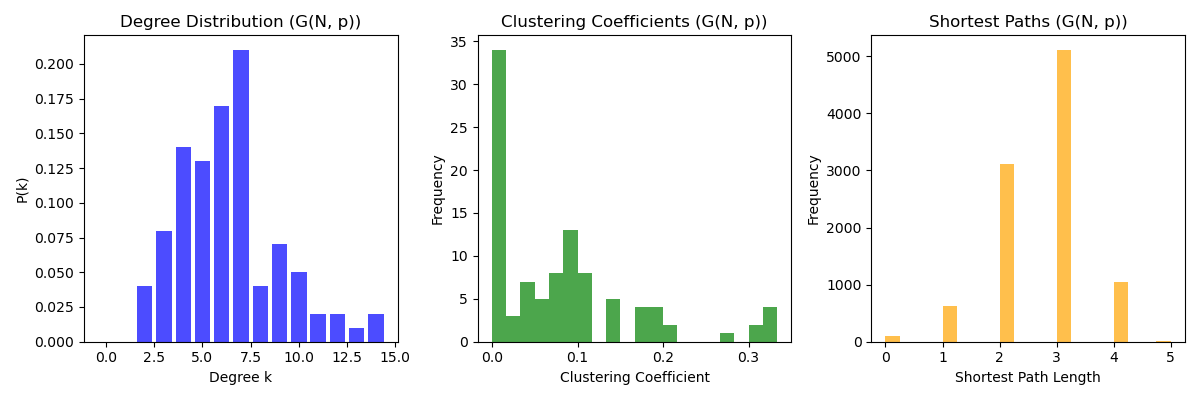
\includegraphics[width=1\textwidth]{../G(N, p)_Graph with 100 nodes and 317 edges.png} % Specify image file and scale
        \caption{N = 100, p = 0.25} % Caption for the image
    \end{figure}
    

    \clearpage

    (c) Watts-Strogatz model WS(N,k,$\beta$) $<$ k $>$ = 2K/N $<$ k $>$ = k, $ 0 < \beta < 1$

    \begin{lstlisting}[style=myPythonStyle, caption={Erdos-Renyi model}]
# Parameters
N = 20  # Number of nodes
k = 4   # Each node is connected to k neighbors
beta = 0.3  # Rewiring probability
G_WS = nx.watts_strogatz_graph(N, k, beta)

# Plotting
plt.figure(figsize=(8, 6))
nx.draw_circular(G_WS, with_labels=True, node_color='lightcoral', edge_color='gray')
plt.title(f"Watts and Strogatz Model WS(N={N}, k={k}, beta={beta})")
plt.savefig('WS.png')
plt.show()

    \end{lstlisting}

    \begin{figure}[htbp!]
        \centering
        \begin{minipage}{0.5\textwidth} % Half the page width for the image
            \centering
            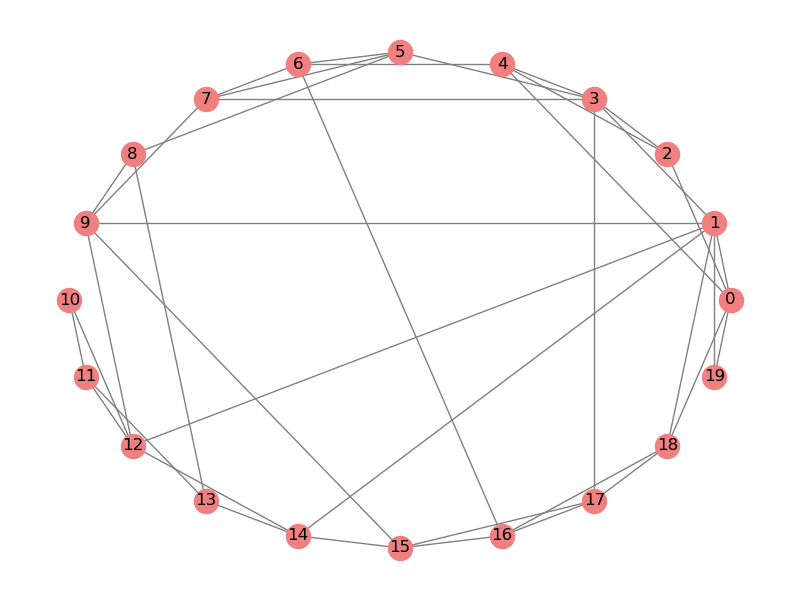
\includegraphics[width=\textwidth]{../WS.png} % Adjust the file path
            \caption{N = 20, k = 4, $\beta = 0.3$}
            \label{fig:ws_graph}
        \end{minipage}%
        \begin{minipage}{0.5\textwidth} % Half the page width for the table
            \centering
            \captionof{table}{Graph Statistics: WS(N, k, $\beta$)}
            \begin{tabular}{|l|c|}
                \hline
                \textbf{Statistic} & \textbf{Value} \\
                \hline
                Average Degree & 6.0 \\
                Average Clustering Coefficient & 0.2203 \\
                Average Path Length & 2.9694 \\
                Diameter & 5 \\
                \hline
            \end{tabular}
            \label{tab:graph_stats}
        \end{minipage}
    \end{figure}
    \begin{figure}[htbp!] % Positioning options: here, top, bottom, page
        \centering
        \includegraphics[width=1\textwidth]{../WS(N, k, β)_Graph with 100 nodes and 300 edges.png} % Specify image file and scale
        \caption{Analysis N = 100, k = 7, $\beta = 0.3$} % Caption for the image
    \end{figure}
    
    
\end{flushleft}


\end{document}
